\begin{frame}
    \frametitle{The International Linear Collider (ILC)}
    \begin{columns}[c,onlytextwidth]
    \begin{column}{0.60\textwidth}
        \begin{itemize}
            \item Linear $e^+e^-$ collider.
            \item Polarized beams.
            \item Initial stage $\sqrt{s} = 250~\GeV$ (considered here).
            \item Upgradable (350~\GeV, 500~\GeV, 1~TeV).
        \end{itemize}
        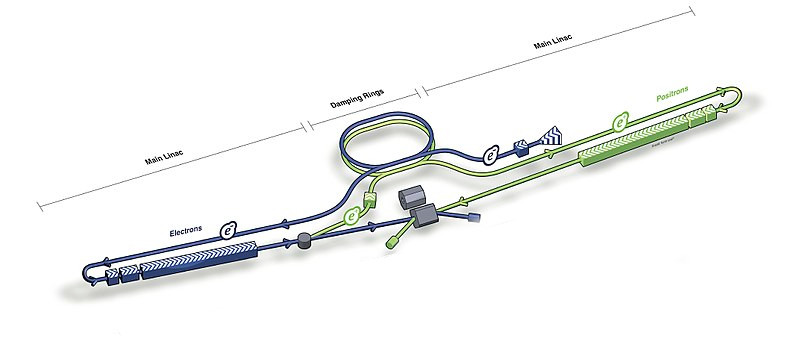
\includegraphics[height=0.4\textheight, width=\textwidth, keepaspectratio]{pr_ILC_SchemeTDR}
    \end{column}
    \begin{column}{0.40\textwidth}
    \begin{tikzpicture}[remember picture,overlay]
        \node[anchor=north west,inner sep=0pt] at ($(current page.center) + (1.5,2.5)$) {
            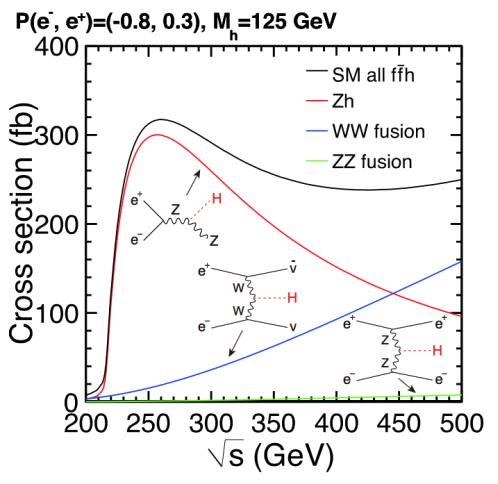
\includegraphics[height=0.6\textheight, width=\textwidth, keepaspectratio]{IGP_xsec_h_ILC_left}
        };
    \end{tikzpicture}
    \end{column}
    \end{columns}
    \vfill
    {\footnotesize
    \href{https://linearcollider.org/technical-design-report/}{ILC Technical Design Report (2013)}\newline
    The International Linear Collider: A Global Project:
    \href{https://arxiv.org/abs/1903.01629}{\emph{\texttt{arXiv:1903.01629}}}
    }
    \end{frame}
